\documentclass[11pt, thmnum, eqsecnum, allcites, dark]{mathbeamer}
%%%%%%%%%%%%%
%% Options %%
%%%%%%%%%%%%%
%% thmnum: numbered theorems
%% eqsecumn: number equaiton with section
%% authoryear: author-year style reference
%% allcites: output all the reference in bib.bib
%% dark: use dark color style
%% light: use light color style
%% nds: not use the default setting

%%%%%%%%%%%%%%%%%%%%%%%%%%%%%%%%%%%%%%%%%%
%===========================
% your definitions:
%===========================
%===================================
%% Self defined command
%===================================
\newcommand{\eps}{\varepsilon}

%===================================
%% Self defined theorem environments
%===================================
%% Note: the following theorem environments
%%       already defined in mathbeamer.cfg
%%       Not need to define it again
%%\theoremstyle{plain}
%%\newtheorem{thm}{Theorem}[section]
%%\newtheorem{lem}[thm]{Lemma}
%%\newtheorem{prop}[thm]{Proposition}
%%\newtheorem{cor}[thm]{Corollary}
%%\theoremstyle{definition}
%%\newtheorem{defn}[thm]{Definition}
%%\theoremstyle{example}
%%\newtheorem{conj}{Conjecture}
%%\newtheorem{exmp}{Example}
%%\newtheorem*{rmk}{Remark}
%%\theoremstyle{break}
%%\newtheorem{bthm}{Theorem}[section]
%%\newtheorem{blem}[thm]{Lemma}
%%\newtheorem{bprop}[thm]{Proposition}
%%\newtheorem{bcor}[thm]{Corollary}

\newcommand{\mthm}{Theorem}


%===========================
% your title/name/institute:
%===========================
\title[\sc Mean Curvature Flow \& Ricci Flow]{\sc On the Evolution of Mean Curvature Flow\\ with Background Ricci Flow}
\author{Stu Name}
\date{\today}
\institute[USTC]{School of Mathematical Sciences, USTC}

\begin{document}
%===========================
% your slides:
%===========================
%\frame[t, allowframebreaks]{\tableofcontents\label{contents}}
%\documentclass[fontset = none, t, aspectratio=169]{ctexbeamer}
\documentclass[fontset = none, t, aspectratio=169]{ctexbeamer}

% 修改自萧山主题的凤岗主题
\usetheme{nwafufengang}

% 载入需要的宏包

\section{Formatting}

\begin{frame}
\frametitle{A First Application Example}
\framesubtitle{Headlines, Table of Contents, simple formatting,
special characters}
\begin{block}{New commands in this section}
\begin{multicols}{2}
\begin{itemize}
  \item \begin{ttfamily}\color{nounibaredII}\textbackslash usepackage\color{black}\{package\}
  \item \color{nounibaredII}\textbackslash command\color{nounibagreenI}[poss\_options]\color{black}\{\\formatted\_text\}
  \item \color{unibablueI}\textbackslash begin\color{black}\{environment\}
  \item \color{unibablueI}\textbackslash end\color{black}\{environment\}
  \item \color{nounibaredII}$\backslash\backslash$\color{black}
  \item \color{nounibaredI}\textbackslash newpage\color{black}
  \item \color{unibablueI}\textbackslash sub$^*$section\color{black}\{Title\}
  \item $\color{nounibaredII}\backslash$\color{nounibaredII}textbf\color{black}\{Text\}
  \item $\color{nounibaredII}\backslash$\color{nounibaredII}textit\color{black}\{Text\}
  \item $\color{nounibaredII}\backslash$\color{nounibaredII}underline\color{black}\{Text\}
  \item \color{nounibaredI}$\color{nounibaredI}\backslash$tiny
  \item \color{nounibaredI}$\color{nounibaredI}\backslash$scriptsize
  \item \color{nounibaredI}$\color{nounibaredI}\backslash$footnotesize
  \item \color{nounibaredI}$\color{nounibaredI}\backslash$normalsize
  \item \color{nounibaredI}$\color{nounibaredI}\backslash$large
  \item \color{nounibaredI}$\color{nounibaredI}\backslash$Large
  \item \color{nounibaredI}$\color{nounibaredI}\backslash$LARGE
  \item \color{nounibaredI}$\color{nounibaredI}\backslash$huge\end{ttfamily}
\end{itemize}
\end{multicols}
\end{block}
\end{frame}


%\begin{frame}
%\frametitle{Ein erstes Anwendungsbeispiel}
%\framesubtitle{Pakete einbinden und Befehle anwenden}
%\begin{itemize}
%  \item Pakete sind Sammlungen von Befehlen oder enthalten z.B. Zeichensätze.\\ Sie werden zu
%  Beginn einer \TeX-Datei angegeben:\\
%  \smallskip
%\textbf{\begin{ttfamily}\color{nounibaredII}\textbackslash usepackage\color{black}\{babel\}
%
%\smallskip
%\end{ttfamily}}
% Einbinden des Paketes „\begin{ttfamily}babel\end{ttfamily}“. (F\"ur Internationalisierung)
%\item Schreibweise von Latex-Befehlen:
%
%\textbf{\begin{ttfamily}\color{nounibaredII}\textbackslash befehl\color{nounibagreenI}[evtl\_optionen]\color{black}\{Formatierter\_Text\}\end{ttfamily}}
%\begin{itemize}
%  \item in \begin{ttfamily}\{\}\end{ttfamily} stehen immer notwendige Parameter bzw. Text
% \item in \begin{ttfamily}[ ]\end{ttfamily} stehen (falls vorhanden)
% zus"atzliche, optionale Parameter
% \item zum Beispiel:
%
%
%\begin{ttfamily}
%\color{nounibaredII}\textbackslash documentclass\color{nounibagreenI}[a4paper,12pt,pdftex,ngerman]\color{black}\{article\}
%\end{ttfamily}
%\end{itemize}
%\end{frame}

\begin{frame}
\frametitle{A First Application Example}
\framesubtitle{Commands cont'd}
\begin{columns}
\begin{column}{0.6\textwidth}
\begin{ttfamily}\scriptsize
\color{nounibaredI}\color{nounibaredI}\textbackslash documentclass\color{black}\color{nounibagreenI}[a4paper, pdftex, ngerman]\color{black}\{article\} \\
\color{nounibaredI}\color{nounibaredI}\textbackslash usepackage\color{black}\color{nounibagreenI}[utf8]\color{black}\{inputenc\} \\
\color{nounibaredI}\color{nounibaredI}\textbackslash usepackage\color{black}\color{nounibagreenI}[T1]\color{black}\{fontenc\} \\
\color{nounibaredI}\color{unibablueI}\textbackslash\color{unibablueI}begin\color{black}\color{black}\{document\} \\
This is a simple document \\
without specials. Line breaks \\
are made automatically! \\
Multiple \\
consecutively blank characters  \\
are condensed to one. \\
Automatic hyphenation.\color{nounibaredI}\color{nounibaredI}\textbackslash \color{nounibaredI}\textbackslash \color{black} \\
Two backslashes make a line \\
break.\color{nounibaredI}\color{nounibaredI}\textbackslash \color{nounibaredI}\textbackslash \color{black} \\
A new paragraph is made by an\\
empty line.\\
\color{nounibaredI}\color{unibablueI}\textbackslash\color{unibablueI}end\color{black}\color{black}\{document\} \\

\end{ttfamily}
\end{column}

\begin{column}{0.4\textwidth}
There are different types of documents.\\ The document type
\begin{ttfamily}article\end{ttfamily} is used here (also possible:
\begin{ttfamily}book\end{ttfamily} and \begin{ttfamily}report\end{ttfamily}). The input in
\begin{ttfamily}[]\end{ttfamily} indicates paper size and font size of the
standard text.\\
%! TODO!
\end{column}
\end{columns}
\end{frame}

\begin{frame}
\frametitle{A First Application Example}
\framesubtitle{Commands cont'd}
\begin{columns}
\begin{column}{0.6\textwidth}
\begin{ttfamily}\scriptsize
\color{nounibaredI}\color{nounibaredI}\textbackslash documentclass\color{black}\color{nounibagreenI}[a4paper, pdftex, ngerman]\color{black}\{article\} \\
\color{nounibaredI}\color{nounibaredI}\textbackslash usepackage\color{black}\color{nounibagreenI}[utf8]\color{black}\{inputenc\} \\
\color{nounibaredI}\color{nounibaredI}\textbackslash usepackage\color{black}\color{nounibagreenI}[T1]\color{black}\{fontenc\} \\
\color{nounibaredI}\color{unibablueI}\textbackslash\color{unibablueI}begin\color{black}\color{black}\{document\} \\
This is a simple document \\
without specials. Line breaks \\
are made automatically! \\
Multiple \\
consecutively blank characters  \\
are condensed to one. \\
Automatic hyphenation.\color{nounibaredI}\color{nounibaredI}\textbackslash \color{nounibaredI}\textbackslash \color{black} \\
Two backslashes make a line \\
break.\color{nounibaredI}\color{nounibaredI}\textbackslash \color{nounibaredI}\textbackslash \color{black} \\
A new paragraph is made by an\\
empty line.\\
\color{nounibaredI}\color{unibablueI}\textbackslash\color{unibablueI}end\color{black}\color{black}\{document\} \\

 \normalsize
\end{ttfamily}
\end{column}
\begin{column}{0.4\textwidth}
\begin{ttfamily}\textbf{\color{unibablueI}\textbackslash begin\color{black}\{environment\}}\end{ttfamily}\\
A new environment begins, in this case the actual document.\\[5mm]

\begin{ttfamily}\textbf{\color{unibablueI}\textbackslash end\color{black}\{environment\}}\end{ttfamily}\\
The environment that started with \begin{ttfamily}\textbf{\color{unibablueI}\textbackslash begin}\color{black}\{\}\end{ttfamily}
ends here.\\[5mm]

\begin{ttfamily}\textbf{\color{nounibaredII}$\backslash\backslash$}\color{black}
~line break\end{ttfamily}\\
\end{column}
\end{columns}
\end{frame}



\begin{frame}
\frametitle{A First Application Example}
\framesubtitle{Packages}
\begin{columns}
\begin{column}{0.6\textwidth}
\begin{ttfamily}\scriptsize
\color{nounibaredI}\color{nounibaredI}\textbackslash documentclass\color{black}\color{nounibagreenI}[a4paper, pdftex, ngerman]\color{black}\{article\} \\
\color{nounibaredI}\color{nounibaredI}\textbackslash usepackage\color{black}\color{nounibagreenI}[utf8]\color{black}\{inputenc\} \\
\color{nounibaredI}\color{nounibaredI}\textbackslash usepackage\color{black}\color{nounibagreenI}[T1]\color{black}\{fontenc\} \\
\color{nounibaredI}\color{unibablueI}\textbackslash\color{unibablueI}begin\color{black}\color{black}\{document\} \\
This is a simple document \\
without specials. Line breaks \\
are made automatically! \\
Multiple \\
consecutively blank characters  \\
are condensed to one. \\
Automatic hyphenation.\color{nounibaredI}\color{nounibaredI}\textbackslash \color{nounibaredI}\textbackslash \color{black} \\
Two backslashes make a line \\
break.\color{nounibaredI}\color{nounibaredI}\textbackslash \color{nounibaredI}\textbackslash \color{black} \\
A new paragraph is made by an\\
empty line.\\
\color{nounibaredI}\color{unibablueI}\textbackslash\color{unibablueI}end\color{black}\color{black}\{document\} \\

 \normalsize
\end{ttfamily}
\end{column}
\begin{column}{0.4\textwidth}
\begin{ttfamily}\textbf{ngerman}\end{ttfamily}\\
The typical formattings and rules of the german language are used (instead of \grqq ngerman\grqq ~you can use \grqq english\grqq ~for english texts).\\[5mm]

\begin{ttfamily}\textbf{inputenc}\end{ttfamily}\\
Defines the character-\\set, that has to be used. You should always use
\begin{ttfamily}UTF-8\end{ttfamily}, because it runs
on all operating systems.\\
\end{column}
\end{columns}
\end{frame}

\begin{frame}
\frametitle{Excursion}
\framesubtitle{Character encoding}
\begin{columns}
\begin{column}{0.6\textwidth}
\image{\textwidth}{image/utf8.png}{UTF-8 in Texmaker}{img:utf8}

\end{column}
\begin{column}{0.4\textwidth}
When you open a document, the correct character set is used automatically.
When you create a new document, it is saved with the default settings 
 of the editor. In the Texmaker settings, the same character set has to be used, that is used in the LaTeX-document.\\
\end{column}
\end{columns}
\textbf{When working in a team, every team member has to set \underline{UTF-8} in
the editor, or problems ar inevitable!} (Broken
vowel mutations, errors during compiling and much more, if there are not only „Windows“-users.)
\end{frame}

\begin{frame}
\frametitle{A First Application Example}
\framesubtitle{As .PDF}
\begin{columns}
\begin{column}{0.5\textwidth}
\begin{ttfamily}\scriptsize
\color{nounibaredI}\color{nounibaredI}\textbackslash documentclass\color{black}\color{nounibagreenI}[a4paper, pdftex, ngerman]\color{black}\{article\} \\
\color{nounibaredI}\color{nounibaredI}\textbackslash usepackage\color{black}\color{nounibagreenI}[utf8]\color{black}\{inputenc\} \\
\color{nounibaredI}\color{nounibaredI}\textbackslash usepackage\color{black}\color{nounibagreenI}[T1]\color{black}\{fontenc\} \\
\color{nounibaredI}\color{unibablueI}\textbackslash\color{unibablueI}begin\color{black}\color{black}\{document\} \\
This is a simple document \\
without specials. Line breaks \\
are made automatically! \\
Multiple \\
consecutively blank characters  \\
are condensed to one. \\
Automatic hyphenation.\color{nounibaredI}\color{nounibaredI}\textbackslash \color{nounibaredI}\textbackslash \color{black} \\
Two backslashes make a line \\
break.\color{nounibaredI}\color{nounibaredI}\textbackslash \color{nounibaredI}\textbackslash \color{black} \\
A new paragraph is made by an\\
empty line.\\
\color{nounibaredI}\color{unibablueI}\textbackslash\color{unibablueI}end\color{black}\color{black}\{document\} \\

 \normalsize
\end{ttfamily}
\end{column}

\begin{column}{0.5\textwidth}
\image{\textwidth}{image/minidocument.png}{The code of the left side as .pdf.}{listing:minidocument}
\end{column}
\end{columns}
\end{frame}



\begin{frame}
\frametitle{Sections}
\framesubtitle{Chapters}
\begin{columns}
\begin{column}{0.5\textwidth}
\begin{ttfamily}\scriptsize
\color{nounibaredI}\color{nounibaredI}\textbackslash documentclass\color{black}\color{nounibagreenI}[a4paper, pdftex, 12pt, ngerman]\color{black}\{article\} \\
\color{nounibaredI}\color{nounibaredI}\textbackslash usepackage\color{black}\color{nounibagreenI}[utf8]\color{black}\{inputenc\} \\
\color{nounibaredI}\color{nounibaredI}\textbackslash usepackage\color{black}\color{nounibagreenI}[T1]\color{black}\{fontenc\} \\
\color{nounibaredI}\color{nounibaredI}\textbackslash usepackage\color{black}\{babel\} \\
\color{nounibaredI}\color{unibablueI}\textbackslash\color{unibablueI}begin\color{black}\color{black}\{document\} \\
\color{nounibaredI}\color{nounibaredI}\textbackslash tableofcontents\color{black} \\
\color{nounibaredI}\color{unibablueI}\textbackslash\color{unibablueI}section\color{black}\color{black}\{Chapter 1\} \\
This is the first part. \\
\color{nounibaredI}\color{unibablueI}\textbackslash\color{unibablueI}subsection\color{black}\color{black}\{Subchapter 1\} \\
The first subchapter. \\
\color{nounibaredI}\color{unibablueI}\textbackslash\color{unibablueI}subsection\color{black}\color{black}\{Subchapter 2\} \\
Another subchapter. \\
\color{nounibaredI}\color{unibablueI}\textbackslash\color{unibablueI}subsubsection\color{black}\color{black}\{Subsubchapter 1\} \\
This is a subchapter of a subchapter. \\
\color{nounibaredI}\color{unibablueI}\textbackslash\color{unibablueI}end\color{black}\color{black}\{document\} \\

\end{ttfamily}
\end{column}
\begin{column}{0.5\textwidth}
\begin{ttfamily}\color{nounibaredI}\textbackslash newpage\color{black}\end{ttfamily}\\
pagebreak\\[3mm]
\begin{ttfamily}\color{unibablueI}\textbackslash section\color{black}\{Title\}\end{ttfamily}\\
A new section begins with the title specified in \begin{ttfamily}\{\}\end{ttfamily}.\\[3mm]
\begin{ttfamily}\color{unibablueI}\textbackslash subsection\color{black}\{Title\}\end{ttfamily}\\
A subsection.\\[3mm]
\begin{ttfamily}\color{unibablueI}\textbackslash subsubsection\color{black}\{Title\}\end{ttfamily}\\
Another level deeper.\\
\end{column}
\end{columns}
\end{frame}

\begin{frame}
\frametitle{Sections}
\framesubtitle{Chapters .PDF}
\begin{columns}
\begin{column}{0.45\textwidth}
\begin{ttfamily}\scriptsize
\color{nounibaredI}\color{nounibaredI}\textbackslash documentclass\color{black}\color{nounibagreenI}[a4paper, pdftex, 12pt, ngerman]\color{black}\{article\} \\
\color{nounibaredI}\color{nounibaredI}\textbackslash usepackage\color{black}\color{nounibagreenI}[utf8]\color{black}\{inputenc\} \\
\color{nounibaredI}\color{nounibaredI}\textbackslash usepackage\color{black}\color{nounibagreenI}[T1]\color{black}\{fontenc\} \\
\color{nounibaredI}\color{nounibaredI}\textbackslash usepackage\color{black}\{babel\} \\
\color{nounibaredI}\color{unibablueI}\textbackslash\color{unibablueI}begin\color{black}\color{black}\{document\} \\
\color{nounibaredI}\color{nounibaredI}\textbackslash tableofcontents\color{black} \\
\color{nounibaredI}\color{unibablueI}\textbackslash\color{unibablueI}section\color{black}\color{black}\{Chapter 1\} \\
This is the first part. \\
\color{nounibaredI}\color{unibablueI}\textbackslash\color{unibablueI}subsection\color{black}\color{black}\{Subchapter 1\} \\
The first subchapter. \\
\color{nounibaredI}\color{unibablueI}\textbackslash\color{unibablueI}subsection\color{black}\color{black}\{Subchapter 2\} \\
Another subchapter. \\
\color{nounibaredI}\color{unibablueI}\textbackslash\color{unibablueI}subsubsection\color{black}\color{black}\{Subsubchapter 1\} \\
This is a subchapter of a subchapter. \\
\color{nounibaredI}\color{unibablueI}\textbackslash\color{unibablueI}end\color{black}\color{black}\{document\} \\

\end{ttfamily}
\end{column}
\begin{column}{0.55\textwidth}
\image{0.7\textwidth}{image/chapters.png}{The chapters are counted automatically}{img:chapters}
\end{column}
\end{columns}
\end{frame}


\begin{frame}
\frametitle{Sections}
\framesubtitle{Part \& Chapter}
Besides \begin{ttfamily}\color{unibablueI}\textbackslash section\color{black}\{\},
\color{unibablueI}\textbackslash subsection\color{black}\{\}\end{ttfamily}, and \begin{ttfamily}\color{unibablueI}\textbackslash subsubsection\color{black}\{\}\end{ttfamily}, there is also the command
 \begin{ttfamily}\color{unibablueI}\textbackslash part\color{black}\{\}\end{ttfamily} which defines a bigger part.
\begin{ttfamily}\color{unibablueI}\textbackslash part\color{black}\{\}\end{ttfamily} fills a whole page on its own.\\
Besides the document type {\ttfamily article}, there are some others for continous
text documents like {\ttfamily book} and {\ttfamily report}.\\
{\ttfamily book} normally distinguishes between left and right side, 
i.e., whether the page number is left or right, and also the other information that can be contained in header and/or footer.
{\ttfamily book} and {\ttfamily report} have the outline
command \begin{ttfamily}\color{unibablueI}\textbackslash chapter\color{black}\{\}\end{ttfamily}.

%\begin{columns}
%\begin{column}{0.5\textwidth}
%CODE
%\end{column}
%\begin{column}{0.5\textwidth}
%OUTPUT
%\end{column}
%\end{columns}
\end{frame}


\begin{frame}
\frametitle{Formattings}
\framesubtitle{Bold, Italic, Underlined}
\begin{columns}
\begin{column}{0.45\textwidth}
\begin{ttfamily}\scriptsize
\color{nounibaredI}\color{nounibaredI}\textbackslash documentclass\color{black}\color{nounibagreenI}[a4paper, pdftex, 12pt, ngerman]\color{black}\{article\} \\
\color{nounibaredI}\color{nounibaredI}\textbackslash usepackage\color{black}\color{nounibagreenI}[utf8]\color{black}\{inputenc\} \\
\color{nounibaredI}\color{nounibaredI}\textbackslash usepackage\color{black}\color{nounibagreenI}[T1]\color{black}\{fontenc\} \\
\color{nounibaredI}\color{unibablueI}\textbackslash\color{unibablueI}begin\color{black}\color{black}\{document\} \\
Among others there are the following options:\color{nounibaredI}\color{nounibaredI}\textbackslash \color{nounibaredI}\textbackslash \color{black} \\
\color{nounibaredI}\color{nounibaredI}\textbackslash textbf\color{black}\{bold\}\color{nounibaredI}\color{nounibaredI}\textbackslash \color{nounibaredI}\textbackslash \color{black} \\
\color{nounibaredI}\color{nounibaredI}\textbackslash textit\color{black}\{italic\}\color{nounibaredI}\color{nounibaredI}\textbackslash \color{nounibaredI}\textbackslash \color{black} \\
\color{nounibaredI}\color{nounibaredI}\textbackslash underline\color{black}\{underlined\}\color{nounibaredI}\color{nounibaredI}\textbackslash \color{nounibaredI}\textbackslash \color{black} \\
\color{nounibaredI}\color{nounibaredI}\textbackslash underline\color{black}\{\color{nounibaredI}\color{nounibaredI}\textbackslash textbf\color{black}\{underlined and bold\}\}\color{nounibaredI}\color{nounibaredI}\textbackslash \color{nounibaredI}\textbackslash \color{black} \\
\color{nounibaredI}\color{unibablueI}\textbackslash\color{unibablueI}end\color{black}\color{black}\{document\} \\

\end{ttfamily}
\end{column}
\begin{column}{0.55\textwidth}
Among others there are the following options:\\[3mm]
\textbf{bold}\\
\textit{italic}\\
\underline{underlined}\\
\underline{\textbf{underlined and bold}}
%\input{formats_pdf.tex}
\begin{block}{Textformatting}
\begin{ttfamily}$\color{nounibaredII}\backslash$\color{nounibaredII}textbf\color{black}\{text\}\end{ttfamily}
bold text\\
\begin{ttfamily}$\color{nounibaredII}\backslash$\color{nounibaredII}textit\color{black}\{text\}\end{ttfamily}
italic text\\
\begin{ttfamily}$\color{nounibaredII}\backslash$\color{nounibaredII}underline\color{black}\{text\}\end{ttfamily}
underlined
\end{block}
\end{column}
\end{columns}
\end{frame}

\begin{frame}
\frametitle{Formattings}
\framesubtitle{Font Size}
\begin{columns}
\begin{column}{0.5\textwidth}
\begin{ttfamily}\scriptsize
\color{nounibaredI}\color{nounibaredI}\textbackslash documentclass\color{black}\color{nounibagreenI}[a4paper, pdftex, 12pt,ngerman]\color{black}\{article\} \\
\color{nounibaredI}\color{nounibaredI}\textbackslash usepackage\color{black}\color{nounibagreenI}[utf8]\color{black}\{inputenc\} \\
\color{nounibaredI}\color{nounibaredI}\textbackslash usepackage\color{black}\color{nounibagreenI}[T1]\color{black}\{fontenc\} \\
\color{nounibaredI}\color{nounibaredI}\textbackslash usepackage\color{black}\{babel\} \\
\color{nounibaredI}\color{unibablueI}\textbackslash\color{unibablueI}begin\color{black}\color{black}\{document\} \\
\color{nounibaredI}\color{nounibaredI}\textbackslash tiny \color{black} illegible text \color{nounibaredI}\color{nounibaredI}\textbackslash \color{nounibaredI}\textbackslash \color{black} \\
\color{nounibaredI}\color{nounibaredI}\textbackslash scriptsize \color{black} very small text\color{nounibaredI}\color{nounibaredI}\textbackslash \color{nounibaredI}\textbackslash \color{black} \\
\color{nounibaredI}\color{nounibaredI}\textbackslash footnotesize \color{black} footnote size \color{nounibaredI}\color{nounibaredI}\textbackslash \color{nounibaredI}\textbackslash \color{black} \\
\color{nounibaredI}\color{nounibaredI}\textbackslash normalsize \color{black} standard size \color{nounibaredI}\color{nounibaredI}\textbackslash \color{nounibaredI}\textbackslash \color{black} \\
\color{nounibaredI}\color{nounibaredI}\textbackslash large \color{black} bigger\color{nounibaredI}\color{nounibaredI}\textbackslash \color{nounibaredI}\textbackslash \color{black} \\
\color{nounibaredI}\color{nounibaredI}\textbackslash Large \color{black} even bigger \color{nounibaredI}\color{nounibaredI}\textbackslash \color{nounibaredI}\textbackslash \color{black} \\
\color{nounibaredI}\color{nounibaredI}\textbackslash LARGE \color{black} very big \color{nounibaredI}\color{nounibaredI}\textbackslash \color{nounibaredI}\textbackslash \color{black} \\
\color{nounibaredI}\color{nounibaredI}\textbackslash huge \color{black} gargantuan \color{nounibaredI}\color{nounibaredI}\textbackslash \color{nounibaredI}\textbackslash \color{black} \\
\color{nounibaredI}\color{unibablueI}\textbackslash\color{unibablueI}end\color{black}\color{black}\{document\} \\

\end{ttfamily}
\end{column}
\begin{column}{0.5\textwidth}
\rm \tiny ~illegible text\\
\scriptsize ~very small text\\
\footnotesize ~footnote size\\
\normalsize ~standard size\\
\large ~bigger\\
\Large ~even bigger\\
\LARGE ~very big\\
\huge  ~gargantuan\\
\end{column}
\end{columns}
\end{frame}

\begin{frame}
\frametitle{Formattings}
\framesubtitle{Bold, Italic, Underlined}
\begin{columns}
\begin{column}{0.5\textwidth}
\begin{ttfamily}\scriptsize\color{nounibaredII}\textbackslash documentclass\color{nounibagreenI}[a4paper, pdftex, 12pt, ngerman]\color{black}\{article\}\\[3mm] 
$\color{nounibaredII}\backslash$\color{nounibaredII}usepackage\color{nounibagreenI}[utf8]\color{black}\{inputenc\}\\
$\color{nounibaredII}\backslash$\color{nounibaredII}usepackage\color{nounibagreenI}[T1]\color{black}\{fontenc\}\\
$\color{nounibaredII}\backslash$\color{nounibaredII}usepackage\color{nounibagreenI}[iso]\color{black}\{umlaute\}\\
$\color{nounibaredII}\backslash$\color{nounibaredII}usepackage\color{black}\{babel\}\\
\color{gray}\% NEU NEU NEU\\
$\color{nounibaredII}\backslash$\color{nounibaredII}usepackage\color{black}\{eurosym\}\\
$\color{unibablueI}\backslash$\color{unibablueI}begin\color{black}\{document\}\\
$\color{nounibaredII}\backslash$\color{nounibaredII}textit\color{black}\{Some
special characters:\}\\
\color{nounibaredII}\textbackslash \% \textbackslash \$ \textbackslash \& \textbackslash \{ \textbackslash \}
\textbackslash \_ \textbackslash \# \textbackslash S \textbackslash copyright\\
\textbackslash slash \~ ~ \color{unibayellowI}\$\color{nounibaredII}$\color{nounibaredII}\backslash$backslash\color{unibayellowI}\$\color{nounibaredII}  ~\textbackslash euro \\

$\color{nounibaredII}\backslash$\color{nounibaredII}textit\color{black}\{hyphen and dash:\} \\
- -- --- \color{unibayellowI}\$\color{black}-\color{unibayellowI}\$\color{black} (the last one is the mathematical minus) \\

$\color{nounibaredII}\backslash$\color{nounibaredII}textit\color{black}\{quotation marks from \begin{ttfamily}ngerman\end{ttfamily}:\} \\
\color{nounibaredII}\textbackslash glqq \textbackslash grqq \textbackslash flqq \textbackslash frqq\\
\color{unibablueI}\textbackslash end\color{black}\{document\}
\end{ttfamily}
\end{column}
\begin{column}{0.5\textwidth}
\textit{Some special characters:}    \\
\% \$ \& \{ \} \_ \# \S ~ \copyright \slash ~ \textbackslash  \euro \\

\textit{hyphen and dash:} \\
- -- --- $-$ (the last one is the mathematical minus) \\

\textit{quotation marks from (n)german:} \\
\glqq \grqq \flqq \frqq\\[5mm]
For the \euro -sign, you need the package \begin{ttfamily}eurosym\end{ttfamily}.\\

\end{column}
\end{columns}
\medskip
\footnotesize Special characters have to be introduced with '\color{nounibaredI}\textbackslash \color{black}'.
Sometimes, e.g. in headlines, vowel mutations from the package ngerman  have to be built with \grqq a \grqq o
\grqq u and \ss ~with \color{nounibaredI} \textbackslash ss \color{black}, for the rest it is sufficient to include the package {\ttfamily babel}.
\end{frame}

% 进行必要的设置
\setbeamercolor*{lower separation line head}{bg=DeepSkyBlue4} 
\setbeamercolor*{normal text}{fg=black,bg=white} 
\setbeamercolor*{alerted text}{fg=red} 
\setbeamercolor*{example text}{fg=black} 
\setbeamercolor*{structure}{fg=DeepSkyBlue4,bg=white} 

\setbeamercolor*{palette tertiary}{fg=black,bg=black!10} 
\setbeamercolor*{palette quaternary}{fg=black,bg=black!10} 

%footline
\setbeamercolor{author in head/foot}{fg=white,bg=}
\setbeamercolor{title in head/foot}{fg=white,bg=}
\setbeamercolor{date in head/foot}{fg=black,bg=}


\makeatletter
\setbeamertemplate{footline}
{%
    \setbox\beamer@tempbox=\hbox{%
        \begin{beamercolorbox}[wd=.333333\paperwidth,ht=2.25ex,dp=1ex,center]{author in head/foot}%
            \usebeamerfont{author in head/foot}\insertshortauthor
        \end{beamercolorbox}%
        \begin{beamercolorbox}[wd=.333333\paperwidth,ht=2.25ex,dp=1ex,center]{title in head/foot}%
            \usebeamerfont{title in head/foot}\insertshorttitle
        \end{beamercolorbox}%
        \begin{beamercolorbox}[wd=.333333\paperwidth,ht=2.25ex,dp=1ex,right]{date in head/foot}%
            \usebeamerfont{date in head/foot}\insertshortdate{}\hspace*{2em}
            \insertframenumber{} / \inserttotalframenumber\hspace*{2ex} 
        \end{beamercolorbox}%
    }%
    \vskip0pt%
        \begin{pgfpicture}{0pt}{0pt}{\paperwidth}{0cm}%
            \usebeamercolor{frametitle right}%
            \pgfpathrectangle{\pgfpointorigin}{\pgfpoint{\paperwidth}{3.5ex}}%
            \pgfusepath{clip}%
            \pgftext[left,base]{\pgfuseshading{beamer@frametitleshade}}%
        \end{pgfpicture}%
    \beamer@tempdim=\ht\beamer@tempbox%
    \advance\beamer@tempdim by 0.95ex%
    \vskip-\beamer@tempdim%
    \box\beamer@tempbox%
    }  
\makeatother


\colorlet{titleright}{yellow!10!white}
\colorlet{titleleft}{DeepSkyBlue4}
\colorlet{titlemid}{green!60!blue}

\makeatletter

\pgfdeclarehorizontalshading[titleleft,titleright]{beamer@frametitleshade}{\paperheight}{%
        color(0pt)=(titleleft);
        color(.5\paperwidth)=(titlemid);
        color(\paperwidth)=(titleright)
}

\AtBeginDocument{
    \pgfdeclareverticalshading{beamer@topshade}{\paperwidth}{%
        color(0pt)=(bg);
        color(4pt)=(black!50!bg)    
    }
}


\renewcommand{\(}{\begin{columns}}
\renewcommand{\)}{\end{columns}}
\newcommand{\<}[1]{\begin{column}{#1}}
\renewcommand{\>}{\end{column}}



% Information
\title[凤岗主题]{\Large 西北农林科技大学 {\LaTeX}  Beamer 主题}

\subtitle{凤岗主题 V\ 2.0}

\author[N. Geng]{耿楠}

\date{\tosemester} % 也可以使用类似\date[2017/04/20]{\zhdate{2017/04/20}}的
              % 方式指定时间

\institute[智能媒体]{智能媒体实验室}

\titlegraphic{%
  \vspace{3.0cm}
  \qrcode[hyperlink, height=1.6cm]{https://github.com/registor/nwafuBeamerTheme}}

\begin{document}

\begin{frame}[plain]
  \maketitle
\end{frame}

\section{简介}

\begin{frame}{简介}{魔改Metropolis主题}
  \begin{itemize}
    \item 改了颜色(用了 \texttt{cncolours.sty})
    \item 加入 \texttt{pgfornament-han} 汉风纹样元素
  \end{itemize}
\end{frame}

\begin{frame}{简介}{为什么叫「凤岗」?}
  \begin{itemize}
    \item 以城市名字命名主题,是 Beamer 的一个传统
    \item 工作在杨凌,北塬上有个地方叫\alert{凤岗}
  \end{itemize}
\end{frame}

\begin{frame}[plain, standout]
作为强调的一个\enquote{standout} 页面
\end{frame}

\section{充版面}

\begin{frame}[allowframebreaks]{区块}{汉风区块结构}

  \begin{block}{Metropolis 走极简风}
    因此「凤岗」主题也走极简风。
  \end{block}

  \begin{exampleblock}{Metropolis 走极简风}
    因此「凤岗」主题也走极简风。
  \end{exampleblock}

  \begin{alertblock}{Metropolis 走极简风}
    因此「凤岗」主题也走极简风。
  \end{alertblock}

  \begin{theorem}[Metropolis 走极简风]
    因此「凤岗」主题也走极简风。
  \end{theorem}

  \begin{proof}[Metropolis 走极简风]
    因此「凤岗」主题也走极简风。
  \end{proof}
\end{frame}

%%%%%%%%%%%%%%%%%%%%%%%%%%%%%% 关于我们 %%%%%%%%%%%%%%%%%%%%%%%%%%%%%%%%%%%
\section[关于我们]{关于我们}
\subsection[联系方式]{联系方式}
\begin{frame}[fragile]{关于我们}{联系方式}
  % colour options
  \definecolor{seplinecolour}{HTML}{357f2d} % green
  \definecolor{iconcolour}{HTML}{2f3142} % dark
  \definecolor{textcolour}{HTML}{2f3142} % dark
  \definecolor{jobtitlecolour}{HTML}{474a65} % light dark

  % define some lengths for internal spacing
  \newlength{\seplinewidth} \setlength{\seplinewidth}{2cm}
  \newlength{\seplineheight} \setlength{\seplineheight}{1pt}
  \newlength{\seplinedistance} \setlength{\seplinedistance}{0.3cm}
  \begin{center}
      \begin{tikzpicture}[font=\small]
      % name
      \matrix[every node/.style={anchor=center,font=\huge},anchor=center] (name) {
        \node{耿\hspace{\ccwd}楠}; \\
        %\node{\color{jobtitlecolour}\normalsize\textit{教授}}; \\
      };
      % sep line 1
      \node[below=0.3\seplinedistance of name] (hl1) {};
      \draw[line width=\seplineheight,color=seplinecolour] (hl1)++(-\seplinewidth/2,0) -- ++(\seplinewidth,0);
      % contact info
      \matrix [below=\seplinedistance of hl1,%
               column 1/.style={anchor=center,color=iconcolour},%
               column 2/.style={anchor=west}] (contact) {
        \node{\faGlobe}; & \node{\url{http://cie.nwsuaf.edu.cn/szdw/}};\\
        \node{\faBuilding}; & \node{西北农林科技大学信息工程学院计算机科学系};\\ 
        \node{\faEnvelope}; & \node{nangeng@nwafu.edu.cn; nangeng@qq.com};\\
        %\node{\faQq}; & \node{970291228};\\
        %\node{\faPhone}; & \node{15829540966}; \\
        \node{\faGithub}; & \node{\url{https://github.com/registor/}}; \\
      };
      sep line 2
      \node[below=\seplinedistance of contact] (hl2) {};
      \draw[line width=\seplineheight,color=seplinecolour] (hl2)++(-\seplinewidth/2,0) -- ++(\seplinewidth,0);
      % interests
      \matrix [below=\seplinedistance of hl2,
         every node/.style={anchor=center,font=\Large}]
         (interests) {
        \node{\faCode}; & \node{\faCoffee}; &
        \node{\faLock}; & \node{\faWrench}; &
        \node{\faCameraRetro}; \\
      };
    \end{tikzpicture}
  \end{center}    
\end{frame}

\begin{frame}[plain, standout]
  感谢聆听!\\
  欢迎多提宝贵意见和建议
\end{frame}

\end{document}

%%% Local Variables:
%%% mode: latex
%%% TeX-master: t
%%% End:


%===========================
% example slides:
%===========================
\section{Lists}
% --------------------------------------------------- Slide --
\subsection{Itemize}
\label{itemize}
\begin{frame}{Lists - Itemize}
  \begin{itemize}
    \item Point A
    \item Point B
    \begin{itemize}
      \item part 1
      \item part 2
    \end{itemize}
    \item Point C
    \item Point D
  \end{itemize}
\end{frame}

% --------------------------------------------------- Slide --
\subsection{Pause}
\label{pause}
\begin{frame}{Lists - Itemize with Pause}
  \begin{itemize}[<+->]
     \item Point A
     \item Point B
    \begin{itemize}
       \item part 1
       \item part 2
    \end{itemize}
     \item Point C
     \item Point D
  \end{itemize}
\end{frame}

% --------------------------------------------------- Slide --
\subsection{Enumerate}
\label{enumerate}
\begin{frame}{Lists - Enumerate}
  \begin{enumerate}
    \item Point A
    \item Point B
    \begin{enumerate}
      \item part 1
      \item part 2
    \end{enumerate}
    \item Point C
    \item Point D
  \end{enumerate}
\end{frame}

% --------------------------------------------------- Slide --
\subsection{Enumerate (Roman Numerals)}
\label{enumerateRomanNumerals}
\begin{frame}{Lists - Enumerate (Roman Numerals)}
  \begin{enumerate} [(I)]
	\item Point A
	\item Point B
	\begin{enumerate} [(i)]
	  \item part 1
      \item part 2
	\end{enumerate}
	\item Point C
	\item Point D
  \end{enumerate}
\end{frame}

\section{Columns}
% --------------------------------------------------- Slide --
\subsection{Columns}
\label{columns}
\begin{frame}{Columns}
  \begin{columns}
    \column{0.5\textwidth}
      Lorem ipsum dolor sit amet, consectetur adipisicing elit, sed do eiusmod tempor incididunt ut labore et dolore magna aliqua.
    \column{0.5\textwidth}
      Lorem ipsum dolor sit amet, consectetur adipisicing elit, sed do eiusmod tempor incididunt ut labore et dolore magna aliqua.
  \end{columns}
\end{frame}

\section{Figures}
% --------------------------------------------------- Slide --
\subsection{Figures}
\label{figures}
\begin{frame}\frametitle{Domination on a Chessboard}
  \begin{figure}[htb]
    \centering
    \begin{tabular}{cc}\pause{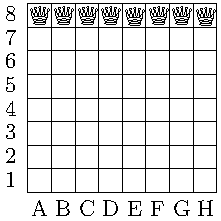
\includegraphics[scale=1]{examples/DomChess8.pdf}}&
      \pause{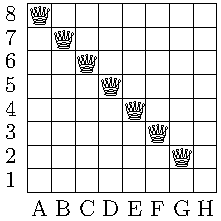
\includegraphics[scale=1]{examples/DomChess7.pdf}}\\
      \pause{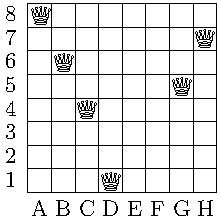
\includegraphics[scale=1]{examples/DomChess6.pdf}}&
      \pause{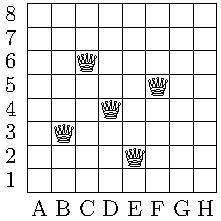
\includegraphics[scale=1]{examples/Chess1.pdf}}
    \end{tabular}
  \end{figure}
\end{frame}

% --------------------------------------------------- Slide --
%\subsection{Figures}
\label{figures2}
\begin{frame}\frametitle{Single figure with caption}
  \begin{figure}[htb]
    \centering
    
\includegraphics[scale=0.25]{examples/figures/400x400.png}
    \caption{This is an caption!}
  \end{figure}
\end{frame}

\section{Description}
% --------------------------------------------------- Slide --
\subsection{Description}
\label{description}
\begin{frame}{Description Environment}
  \begin{description}
    \item[API] Application Programming Interface
    \item[LAN] Local Area Network
    \item[ASCII] American Standard Code for Information Interchange
  \end{description}
\end{frame}

%\section{Tables}
% --------------------------------------------------- Slide --
%\subsection{Tables}
\label{tables}
\begin{frame}\frametitle{Tables}
  \begin{table}
    \begin{tabular}{l | c | c | c | c }
      Competitor Name & Swim & Cycle & Run & Total \\
      \hline \hline
      John T & 13:04 & 24:15 & 18:34 & 55:53 \\ 
      Norman P & 8:00 & 22:45 & 23:02 & 53:47\\
      Alex K & 14:00 & 28:00 & n/a & n/a\\
      Sarah H & 9:22 & 21:10 & 24:03 & 54:35 
    \end{tabular}
    \caption{Triathlon results}
  \end{table}
\end{frame}
%\section{Blocks}
% --------------------------------------------------- Slide --
%\subsection{Blocks}
\label{blocks}
\begin{frame}\frametitle{Blocks}
  \begin{block}{Block Title}
    Lorem ipsum dolor sit amet, consectetur adipisicing elit, sed do eiusmod tempor incididunt ut labore et dolore magna aliqua.
  \end{block}
  \begin{alertblock}{Alert Block Title}
    Lorem ipsum dolor sit amet, consectetur adipisicing elit, sed do eiusmod tempor incididunt ut labore et dolore magna aliqua.
  \end{alertblock}
\end{frame}
% -*- coding: utf-8 -*-
\section{Definition}
% --------------------------------------------------- Slide --
\subsection{Definition}
\label{definition}
\begin{frame}{Definition}
  Then there’s the definition environment which produces a standard color block but with the title already specified as ‘definition’.
  \begin{semiverbatim}
    \\begin\{definition\}\newline
    A prime number is a number that...\newline
    \\end\{definition\}
  \end{semiverbatim}
  \begin{definition}
    A prime number is a number that...
  \end{definition}
\end{frame}
\subsection{Custom definition}
\begin{frame}{Custom definition}
  You can also use the custom definition defined in ``slides/usrdef.tex'', for example
  \begin{semiverbatim}
    \\begin\{defn\}\newline
    A prime number is a number that...\newline
    \\end\{defn\}
  \end{semiverbatim}
  \begin{defn}
    A prime number is a number that...
  \end{defn}
\end{frame}

\documentclass{beamer}
\usepackage[utf8]{inputenc}
\usepackage[T1]{fontenc}
\usepackage{lipsum, lmodern}
\usetheme{Klope} % or Median, or Metro, or PraterStreet, or Milano

\author{Author Name}
\title{Beamer presentation}
\institute{Pázmány Péter Catholic University}
\date{\today}

\begin{document}
\frame{\maketitle}
\begin{frame}{Table of contents}
	\tableofcontents
\end{frame}

\section{Introduction}
\begin{frame}{Itemize}
\begin{itemize}
\item Here you can see an itemization
\begin{itemize}
\item It has items
\begin{itemize}
\item The items are below each other
\end{itemize}
\end{itemize}
\end{itemize}
\end{frame}

\begin{frame}{Enumerate}
\begin{enumerate}
\item Here you can see an enumeration
\item It has items
\item The items are numbered
\end{enumerate}
\[
	f(x)=\sum_{i=0}^\infty \frac{f^{(i)}(x_0)}{i!}(x-x_0)^i
\]
\end{frame}

\begin{frame}{Theorems and environments}
\begin{theorem}[Sample theorem]
This presentation is essentially useless.
\end{theorem}
\begin{proof}
This proof is essentially incorrect.
\end{proof}
\end{frame}

\begin{frame}{Example slide with Title}
\begin{example}
Major problem.
\end{example}
\begin{solution}
Minor nuisance.
\end{solution}
\end{frame}

\begin{frame}[plain]{Plain frame with title}
\lipsum[1]
\end{frame}
\end{document}
%\section{Theorem}
% --------------------------------------------------- Slide --
%\subsection{Theorem Code}
\label{theoremCode}
\begin{frame}\frametitle{Theorem}
  There is also a group of blocks that are especially useful for presenting mathematics. For example the ‘theorem’ environment, the ‘corollary’ environment and the ‘proof’ environment.
  \begin{semiverbatim}
    \\begin\{theorem\}[Pythagoras] \newline
      $ a^2 + b^2 = c^2$ \newline
    \\end\{theorem\} \newline
    \\begin\{corollary\} \newline
      $ x + y = y + x  $ \newline
    \\end\{corollary\} \newline
    \\begin\{proof\} \newline
      $\omega +\phi = \epsilon $ \newline
    \\end\{proof\}
  \end{semiverbatim}
\end{frame}

% --------------------------------------------------- Slide --
%\subsection{Theorem Blocks}
\label{theoremBlocks}
\begin{frame}\frametitle{Theorem Blocks}
  \begin{theorem}[Pythagoras] 
    $ a^2 + b^2 = c^2$
  \end{theorem}
  \begin{corollary}
    $ x + y = y + x  $
  \end{corollary}
  \begin{proof}
    $\omega +\phi = \epsilon $
  \end{proof}
\end{frame}
\section{Hyperlinks}
% --------------------------------------------------- Slide --
\subsection{Hyperlinks Code}
\label{hyperlinks}
\begin{frame}{Hyperlink}
Before we can create any hyperlinks we need to tag the frames we want to link to using the \label command.

\hyperlink{contents}{click here}
\hyperlink{section1}{\beamerbutton{section 1 page}}
\hyperlink{columns}{\beamergotobutton{columns page}}
\hyperlink{figures}{\beamerskipbutton{pictures page}}
\hyperlink{figures}{\beamerreturnbutton{pictures page}}

\end{frame}


%===========================
% bibliography
%===========================
%input "slides/bib.bib"
\end{document}
